\documentclass[10pt,a4paper,twocolumn]{article}
\usepackage[utf8]{inputenc}
\usepackage[german]{babel}
\usepackage{amsmath}
\usepackage{amsfonts}
\usepackage{amssymb}
\usepackage{fancyhdr}
\usepackage{lastpage}
\usepackage{graphicx}
\usepackage[cm]{fullpage}
\usepackage{color}
\usepackage{framed}

% Used for indicator function
\usepackage{bbm}

\pagestyle{fancy}
\fancyhf{}
\renewcommand{\headrulewidth}{0pt}
\renewcommand{\footrulewidth}{0pt}
\fancyfoot[C]{\thepage/\pageref{LastPage}}
\setlength{\parindent}{0in} 

\begin{document}

\begin{center}
\textbf{Zusammenfassung\\ Wahrscheinlichkeit und Statistik}

\vspace{10pt}

\textbf{Autor:}\\
André Gasser, gassera@student.ethz.ch

\vspace{10pt}

\textbf{Datum:}\\
Januar 2013
\end{center}

\section{Kombinatorik}

\subsection{Permutation}
n unterschiedlichen Kugeln:
\[
P(n)=n!
\]

n unterschiedliche Kugeln mit $n_1,n_2,...,n_k$ gleichen Kugeln:
\[
P(n,n_1,n_2,...,n_k)=\frac{n!}{n_1!n_2!...n_k!}
\]

\textbf{Bemerkungen:}
\begin{itemize}
\item Ermitteln der Anzahl Anordnungen.
\end{itemize}

\subsection{Kombination}
Mit Zurücklegen:
\[
C_w(n,k)=\left( 
	\begin{array}{c}
		n+k-1 \\
		k
	\end{array}
\right) =
\frac{(n+k-1)!}{k!(n-1)!}
\]

Ohne Zurücklegen:
\[
C(n,k)=\left( 
	\begin{array}{c}
		n \\
		k
	\end{array}
\right) =
\frac{n!}{k!(n-k)!}
\]

\textbf{Bemerkungen:}
\begin{itemize}
\item Reihenfolge spielt keine Rolle.
\end{itemize}

\subsection{Variation}
Mit Zurücklegen:
\[
V_w(n,k)=n^k
\]

Ohne Zurücklegen:
\[
V(n,k)=\frac{n!}{(n-k)!}
\]

\textbf{Bemerkungen:}
\begin{itemize}
\item Reihenfolge ist wesentlich.
\end{itemize}

\section{Wahrscheinlichkeit}

\subsection{Allgemeine Rechenregeln}
\[
\begin{array}{rcl}
	P\left[A^C\right] & = & 1-P[A] \\
	P\left[\Omega\right] & = & P[A]+P\left[A^C\right]=1 \\
	P[\emptyset] & = & 0 \\
	P\left[B^C|A\right] & = & 1-P[B|A] \\
	A\subseteq B & \Rightarrow & P[A] \leq P[B] \\
\end{array}
\]

\subsection{DeMorgan'sche Gesetze}
\[
\begin{array}{rcl}
	\overline{A\cap B} & = & \overline{A}\cup\overline{B} \\
	\overline{A\cup B} & = & \overline{A}\cap\overline{B}\\
\end{array}
\]

\subsection{Additionssatz}
Zur Berechnung der Wahrscheinlichkeit, dass Ereignis $A$ oder $B$ eintritt.

\vspace{10pt}

Allgemein:
\[
P[A \cup B] = P[A] + P[B] - P[A \cap B]
\]

A,B disjunkt:
\[
P[A \cup B] = P[A] + P[B]
\]

\textbf{Bemerkungen:}
\begin{itemize}
\item Wenn die Ereignisse nicht offensichtlich disjunkt sind, die \textbf{erste Formel verwenden}!
\end{itemize}

\subsection{Multiplikationssatz}
Zur Berechnung der Wahrscheinlichkeit, dass die Ereignisse $A$ und $B$ eintreten.
\[
P[A \cap B] = P[A] \cdot P[B|A]
\]

\textbf{Bemerkungen}
\begin{itemize}
\item $P[A,B]=P[A \cap B]$.
\end{itemize}

\subsection{Bedingte Wahrscheinlichkeit}
Die bedingte Wahrscheinlichkeit von B gegeben A entspricht der Wahrscheinlichkeit, dass B eintritt, wenn man schon weiss, dass A eingetreten ist. Es gilt:
\[
P[B|A]=\frac{P[A\cap B]}{P[A]}
\]
\[
P[A\cap B]=P[A]\cdot P[B|A]=P[B]\cdot P[A|B]
\]

\textbf{Bemerkungen:}
\begin{itemize}
\item Die \textbf{Pfadregel}, nach der Wahrscheinlichkeiten in einem \textbf{Wahrscheinlichkeitsbaum} multipliziert werden, um die Wahrscheinlichkeit eines Blattes zu erhalten, entspricht einer Verkettung bedingter Wahrscheinlichkeiten.
\end{itemize}

\subsubsection{Satz der totalen Wahrscheinlichkeit}
\[
P[B] = \sum \limits_{i=1}^{n} P[A_i] \cdot P[B|A_i]
\]

\subsubsection{Satz von Bayes}
Zur Berechnung einer bestimmten Zwischenstation $A_k$ in einem Ereignisbaum, wobei mehrere Ereignisse $A_i$ zu Ereignis $B$ führen.
\[
P[A_k|B] = \frac{P[A_k] \cdot P[B|A_k]}{\sum \limits_{i=1}^{n} P[A_i] \cdot P[B|A_i]}
\]

\subsection{Eigenschaften von Ereignissen}

\subsubsection{Unabhängigkeit}
Wenn zwischen zwei Ereignissen $A$ und $B$ kein kausaler Zusammenhang besteht (d.h. es gibt keine gemeinsamen Ursachen oder Ausschliessungen), dann sind sie \emph{unabhängig} voneinander. In diesem Fall gilt:
\[
P[A \cap B] = P[A] \cdot P[B]
\]

\section{Zufallsvariablen}

\subsection{Diskrete Zufallsvariablen}

\subsubsection{Gewichtsfunktion}
Die Summe aller Gewichte ist immer 1 und die Werte immer im Intervall [0,1]:
\[
\sum\limits_{i=1}^{\infty}f(x)=1
\]
\subsubsection{Verteilungsfunktion}

\subsection{Stetige Zufallsvariablen}

\subsubsection{Dichtefunktion}

Die Fläche unter der Dichtefunktion ist immer 1 und die Werte immer im Intervall [0,1]: 
\[
\int\limits_{-\infty}^{\infty}f(x)dx=1
\]

\textbf{Bemerkungen}
\begin{itemize}
\item Durch Integrieren der Dichtefunktion erhält man die Verteilungsfunktion.
\end{itemize}

\subsubsection{Verteilungsfunktion}
\[
F(x) = P[X \leq x] = \int\limits_{-\infty}^{x}f(u)du
\]

\textbf{Bemerkungen}
\begin{itemize}
\item Durch Ableiten der Verteilungsfunktion erhält man die Dichtefunktion.
\end{itemize}

\subsection{Gemeinsame Verteilungen}

\textbf{Gemeinsame Verteilungsfunktion:} Die gemeinsame Verteilungsfunktion von $n$ Zufallsvariablen $X_1,...,X_n$ ist die Abbildung $F:\mathbb{R}^n\rightarrow [0,1]$,
\[
F(t_1,...,t_n):=P[X_1\leq t_1,...,X_n\leq t_n]
\]

\textbf{Gemeinsame Gewichtsfunktion:} Falls $X_1,...,X_n$ \emph{diskrete} Zufallsvariablen sind, ist ihre gemeinsame Gewichtsfunktion $p:\mathbb{R}^n\rightarrow [0,1]$ definiert durch
\[
p(x_1,...,x_n):=P[X_1=x_1,...,X_n=x_n]
\]

\textbf{Gemeinsame Dichte:} Seien $X_1,...,X_n$ \emph{stetige} Zufallsvariablen mit gemeinsamer Verteilungsfunktion $F(t_1,...,t_n)$. Die Funktion $f:\mathbb{R}^n\rightarrow [0,\infty)$ heisst \emph{gemeinsame Dichte} von $X_1,...,X_n$, falls für alle $t_i\in\mathbb{R}$ gilt
\[
F(t_1,...,t_n)=\int\limits_{-\infty}^{t_1}...\int\limits_{-\infty}^{t_n}f(x_1,...,x_n)\ dx_n...dx_1
\]

\subsubsection{Randverteilungen}
Seien $X$ und $Y$ Zufallsvariablen mit gemeinsamer Verteilungsfunktion $F_{XY}$, dann ist die Randverteilung $F_X:\mathbb{R}\rightarrow [0,1]$ von $X$ definiert durch
\[
F_X=P[X\leq x]=P[X\leq x,Y\leq\infty]=\lim_{y\to\infty}F_{XY}(x,y)
\]

Für zwei \emph{diskrete} Zufallsvariablen $X$ und $Y$ mit gemeinsamer Gewichtsfunktion $f_{XY}(x,y)$ ist die Gewichtsfunktion der Randverteilung von $X$ gegeben durch
\[
f_X=P[X=x]=\sum\limits_{j}P[X=x,Y=y_j]=\sum\limits_{j}f_{XY}(x,y_j)
\]

Für zwei \emph{stetige} Zufallsvariablen $X$ und $Y$ mit gemeinsamer Dichte $f_{XY}(x,y)$ ist die Dichtefunktion der Randverteilung (Randdichte) von $X$ gegeben durch
\[
f_X(x)=\int\limits_{\infty}^{\infty}f_{XY}(x,y)\ dy
\]

\subsubsection{Bedingte Verteilung}
\textbf{Bedingte Gewichtsfunktion:} Seien $X$ und $Y$ \emph{diskrete} Zufallsvariablen mit gemeinsamer Gewichtsfunktion $f_{XY}(x,y)$, dann ist die bedingte Gewichtsfunktion $f_{X|Y}(x|y)$ von $X$ gegeben $Y$ definiert durch
\[
f_{X|Y}(x|y)=P[X=x|Y=y]=\frac{f_{XY}(x,y)}{f_Y(y)}
\]

\textbf{Bedingte Dichte:} Für zwei \emph{stetige} Zufallsvariablen $X$ und $Y$ mit gemeinsamer Dichte $f_{XY}(x,y)$ ist die bedingte Dichte $f_{X|Y}$ von $X$ gegeben $Y$ definiert durch
\[
f_{X|Y}(x|y)=\frac{f_{XY}(x,y)}{f_Y(y)}
\]

\subsection{Funktionen diskreter Zufallsvariablen}

\subsubsection{Summe von Zufallsvariablen}
...

\subsubsection{Produkte von Zufallsvariablen}
...

\subsection{Funktionen stetiger Zufallsvariablen}
\[
\begin{array}{rcl}
	Y=aX+b & = & F_Y(t)=P[Y\leq t]=P[aX+b\leq t] \\
	& = & P[X\leq \frac{t-b}{a}]=F_X(\frac{t-b}{a}) \\
	Y=X^2 & = & F_Y(t)=P[Y\leq t]=P[X^2\leq t] \\
	& = & P[-\sqrt{t}\leq t\leq\sqrt{t}]=F_X(\sqrt{t})-F_X(-\sqrt{t}) \\
	Y=\frac{1}{X} & = & F_Y(t)=P[Y\leq t]=P[\frac{1}{X}\leq t] \\
	& = & P[X\geq\frac{1}{t}]=1-P[X\leq\frac{1}{t}]=1-F_X(\frac{1}{t})
\end{array}
\]

\subsection{Chebyshev-Ungleichung}
Die Chebyshev-Ungleichung liefert eine Abschätzung von Wahrscheinlichkeiten, auch wenn die genaue Verteilungsfunktion nicht bekannt ist. Es muss nur der Erwartungswert $E[X]$ und die Varianz $Var[X] < \infty$ einer Zufallsvariablen $X$ bekannt sein, dann gilt für jedes $k > 0$:
\[
P\left[|X - E[X]| \geq k \right] \leq \frac{Var[X]}{k^2}
\]

\subsection{Eigenschaften von Zufallsvariablen}

\subsubsection{Unabhängigkeit}
Zwei Zufallsvariablen $X$ und $Y$ heissen unabhängig, wenn stets gilt
\[
\begin{array}{rcl}
	F(x,y) & = & F_X(x) \cdot F_Y(y) \\
	f(x,y) & = & f_X(x) \cdot F_Y(y) \\
\end{array}
\]
wobei $F_X(x), F_X(y)$ die Verteilungsfunktionen und $f_X(x), f_Y(y)$ die Gewichts- bzw. Dichtefunktionen von $X$ und $Y$ sind.

\subsubsection{Unkorreliert}
Zwei Zufallsvariablen $X$ und $Y$ heissen \emph{unkorreliert}, falls gilt $Cov(X,Y)=0$.

Eine Menge von Zufallsvariablen $X_1,X_2,...,X_n$ heissen \emph{paarweise unkorreliert}, wenn alle Paare $X_i,X_j$ mit $i\neq j$ unkorreliert sind.

\subsection{Erwartungswert}
Der Erwartungswert ist das langfristige Durchschnittsergebnis bei einem Zufallsexperiment mit vielen Wiederholungen.

\vspace{10pt}

Diskrete Verteilung:
\[
E[X]=\sum\limits_{i} x_i\cdot f(x_i)
\]

Stetige Verteilung:
\[
E[X]=\int\limits_{-\infty}^{\infty}x\cdot f(x)dx
\]

\subsubsection{Additionssatz für Erwartungswerte}
Der Erwartungswert einer aus $n$ (diskreten oder stetigen) Zufallsvariablen $X_1,X_2,...,X_n$ gebildeten Summe
\[
Z=a_1X_1+a_2X_2+...+a_nX_n
\]
ist gleich der Summe der Erwartungswerte der einzelnen Zufallsvariablen:
\[
E[Z]=a_1E[X_1]+a_2E[X_2]+...+a_nE[X_n]
\]

\subsubsection{Multiplikationssatz für Erwartungswerte}
Der Erwartungswert eines aus $n$ \emph{stochastisch unabhängigen} (diskreten oder stetigen) Zufallsvariablen $X_1,X_2,...,X_n$ gebildeten Produkts
\[
Z=X_1\cdot X_2\cdot ...\cdot X_n
\]
ist gleich dem Produkt der Erwartungswerte der einzelnen Zufallsvariablen:
\[
E[Z]=E[X_1\cdot X_2\cdot ...\cdot X_n]=E[X_1]\cdot E[X_2]\cdot ...\cdot E[X_n]
\]

\subsubsection{Formeln für 2. Moment}
Dieses wird z.B. für die Momenten-Methode und zur Berechnung der Varianz benötigt.

\vspace{10pt}

Diskrete Verteilung:
\[
E[X^2]=\sum\limits_{i} x_i^2\cdot f(x_i)
\]

Stetige Verteilung:
\[
E[X^2]=\int\limits_{-\infty}^{\infty}x^2\cdot f(x)dx
\]

\subsubsection{Weitere Rechenregeln}
\[
\begin{array}{rcl}
	E[a] & = & a \text{(für a = const.)} \\
	E[aX] & = & a \cdot E[X] \text{(für a = const.)} \\
	E[aX + b] & = & a \cdot E[X] + b \\	
	E[E[X]] & = & E[X] \\
\end{array}
\]

\subsection{Varianz}
Die Varianz ist ein Streuungsmass, also ein Mass für die Abweichung einer Zufallsvariable von ihrem Erwartungswert.

\vspace{10pt}

Diskrete Verteilung:
\[
Var[X]=\sum\limits_{i}(x_i-E[X])^2\cdot f(x_i)
\]

Stetige Verteilung:
\[
Var[X]=\int\limits_{-\infty}^{\infty}(x-E[X])^2\cdot f(x)dx
\]

Vereinfachte Berechnung:
\[
\begin{array}{c}
	Var[X] = E[X^2] - E[X]^2 \\
\end{array}
\]

\subsubsection{Additionssatz für Varianzen}
Die Varianz einer aus $n$ \emph{stochastisch unabhängigen} (diskreten oder stetigen) Zufallsvariablen $X_1,X_2,...,X_n$ gebildeten Summe
\[
Z=a_1X_1+a_2X_2+...+a_nX_n
\]
ist gleich der Summe der Varianzen der einzelnen Zufallsvariablen:
\[
Var[Z]=a_1^2Var[X_1]+a_2^2Var[X_2]+...+a_n^2Var[X_n]
\]

\subsubsection{Weitere Rechenregeln}
\[
\begin{array}{rcl}
	Var[aX + b] & = & a^2 \cdot Var[X] \\
	Var[aX + bY] & = & a^2 \cdot Var[X] + b^2 \cdot Var[Y] + \\
	& &  2ab \cdot Cov[X,Y] \\
\end{array}	
\]

\subsection{Kovarianz}
Die Kovarianz ist ein Mass für den Zusammenhang zwischen zwei Zufallsvariablen $X$ und $Y$ bzw. der Streuung zwischen ihnen.
\[
\begin{array}{rcl}
	Cov[X,Y] & = & E[(X - E[X])(Y - E[Y])] \\
	Cov[X,Y] & = & E[XY] - E[X] \cdot E[Y] \\
	Cov[X,Y] & = & \frac{1}{2} \cdot \left(Var[X + Y] - Var[X] - Var[Y] \right)	\\
	Cov[X,Y] &= & Cov[Y,X] \\
	Cov[X,X] & = & Var[X] \\
	Cov[aX + b,Y] & = & a \cdot Cov[X,Y] \\
	Cov[X + Y,Z] & = & Cov[X,Z] + Cov[Y,Z] \\
	\forall a \in \mathbb{R}: Cov[X,a] & = & 0 \\
	\forall b \in \mathbb{R}: Cov[X,bY] & = & b \cdot Cov[X,Y] \\
\end{array}
\]

\subsection{Standardabweichung}
\[
sd[X] = \sqrt{Var[X]}
\]

\section{Indikatorfunktion $\mathbbm{1}$}
Die Indikatorfunktion ist eine spezielle Zufallsvariable, welche angibt ob ein Ereignis A eingetreten ist.
\begin{equation}
	\mathbbm{1}_A(\omega) = \begin{cases}
			1 & \omega \in A\\
			0 & \omega \not\in A
		\end{cases}
\end{equation}


\section{Diskrete Verteilungen}

\subsection{Bernoulli-Verteilung}
Verteilung eines Experiments mit zwei Ausgängen (Erfolg, Misserfolg) mit Erfolgsparameter $p$.

\vspace{10pt}

Notation:
\[
X \sim Be(p)
\]

Gewichtsfunktion:
\[
f(x)=P[X=x]=p^x\cdot (1-p)^{1-x}
\]

Erwartungswert:
\[
E[X]=p
\]

Varianz:
\[
Var[X]=p(1-p)
\]

\textbf{Beispiel (Münzwurf):} Ein fairer Münzwurf ist bernoulliverteilt mit Parameter $p=\frac{1}{2}$. Für einen Parameter $p\neq\frac{1}{2}$ wäre der Münzwurf unfair.

\subsection{Binomial-Verteilung}
Beschreibt die Anzahl der Erfolge in einer Serie von \emph{gleichartigen} und \emph{unabhängigen} Versuchen, die jeweils genau zwei mögliche Ergebnisse haben (''Erfolg'' oder ''Misserfolg''). $n$ ist die Anzahl der Versuche bzw. Wiederholungen, $p$ ist die Wahrscheinlichkeit für einen "Erfolg".

\vspace{10pt}

Notation:
\[
X \sim Bin(n,p)
\]

Gewichtsfunktion:
\[
f(x)=P[X=x]=
\left(
	\begin{array}{c}
		n \\
		x
	\end{array}
\right)
p^x(1-p)^{n-x}
\]

Verteilungsfunktion:
\[
F(x)=P[X \leq x]=\sum \limits_{k=0}^x 
\left(
	\begin{array}{c}
		n \\
		k
	\end{array}
\right)
p^k(1-p)^{n-k}
\]

Erwartungswert:
\[
E[X]=np
\]

Varianz:
\[
Var[X]=np(1-p)
\]

\textbf{Bemerkungen:}
\begin{itemize}
\item Die Binomialverteilung $Bin(n,p)$ darf für grosse $n$ und kleine $p$ näherungsweise durch die Poisson-Verteilung mit Parameter $\lambda = np$ ersetzt werden (Faustregel: $np<10$ und $n>1500p$).
\end{itemize}

\textbf{Beispiel:} Geburtstagsproblem, Anzahl der Köpfe beim 10-maligen Münzwurf.

\subsection{Geometrische Verteilung}
Wartezeit auf ersten Erfolg bei einer Folge von 0-1-Experimenten mit Erfolgsparameter $p$. $X$ ist die Nummer des ersten erfolgreichen Experiments.

\vspace{10pt}

Notation:
\[
X \sim Geom(p)
\]

Gewichtsfunktion:
\[
f(x)=P[X=x]=p(1-p)^{x-1}
\]

Verteilungsfunktion:
\[
F(x)=P[X \leq x]=1-(1-p)^{x}
\]

Erwartungswert:
\[
E[X]=\frac{1}{p}
\]

Varianz:
\[
Var[X]=\frac{1-p}{p^2}
\]

\textbf{Beispiel:} Wartezeit auf Kopf bei wiederholtem Münzwurf

\subsection{Poisson-Verteilung}
Ereignet sich in einem Intervall (z.B. in einer gewissen Zeit, auf einer gewissen Fläche, in einem gewissen Volumen, usw.) ein völlig zufällig auftretendes Ereignis im Schnitt $\mu$ mal (Erwartungswert), dann ist die Zufallsgrösse, welche die Häufigkeit des Ereignisses in diesem Intervall angibt, poissonverteilt mit Parameter $\lambda=\mu$.

\vspace{10pt}

Notation:
\[
X \sim P(\lambda), X \sim Pois(\lambda)
\]

Gewichtsfunktion:
\[
f(x)=P[X=x]=e^{-\lambda}\frac{\lambda^{x}}{x!}
\]

Verteilungsfunktion:
\[
F(x)=P[X \leq x]=e^{-\lambda}\sum \limits_{k=0}^x \frac{\lambda^{k}}{k!}
\]

Erwartungswert:
\[
E[X]=\lambda
\]

Varianz:
\[
Var[X]=\lambda
\]

\textbf{Bemerkungen}
\begin{itemize}
\item Falls $Z=X+Y$ und $X\sim Pois(\lambda)$, $Y\sim Pois(\mu)$ dann gilt $Z\sim Pois(\lambda+\mu)$.
\end{itemize}

\textbf{Beispiel:} Anzahl eingehender Druckaufträge in $n=3600$ Sekunden mit einer Jobwahrscheinlichkeit von $p=1\%$ pro Sekunde, wenn pro Sekunde maximal ein Job eintreffen kann.

\subsection{Negativbinomiale Verteilung}
Wartezeit auf den $r$-ten Erfolg bei einer Folge von unabhängigen 0-1-Experimenten mit Erfolgsparameter $p$.

Notation:
\[
X \sim NB(r,p)
\]

Gewichtsfunktion:
\[
f(x)=P[X=x]=\left(
	\begin{array}{c}
		x-1 \\
		r-1
	\end{array}
\right)p^{r}(1-p)^{x-r}
\]

Verteilungsfunktion:
\[
F(x)=P[X \leq x]=\sum \limits_{i=r}^x
\left(
	\begin{array}{c}
		i-1 \\
		r-1
	\end{array}
\right)p^{r}(1-p)^{i-r}
\]

Erwartungswert:
\[
E[X]=\frac{r}{p}
\]

Varianz:
\[
Var[X]=\frac{r(1-p)}{p^2}
\]

\textbf{Beispiel:} Wartezeit auf dritten Kopf beim wiederholten Münzwurf

\subsection{Hypergeometrische Verteilung}
Urnenmodell für Ziehen ohne Zurücklegen. In einer Urne befinden sich $n$ Gegenstände. Davon sind $r$ Gegenstände vom Typ A und $n-r$ Gegenstände vom Typ B. Es werden $m$ Gegenstände ohne Zurücklegen gezogen. $X$ beschreibt die Wahrscheinlichkeitsverteilung für die Anzahl $k$ der Gegenstände vom Typ A in der Stichprobe.

\vspace{10pt}

Notation:
\[
X \sim HypGeom(n,m,r)
\]

Gewichtsfunktion:
\[
f(x)=P[X=x]=\frac{
\left(
	\begin{array}{c}
		r \\ x
	\end{array}
\right)
\left(
	\begin{array}{c}
		n-r \\ m-x
	\end{array}
\right)
}{
\left(
	\begin{array}{c}
		n \\ m
	\end{array}
\right)
}
\]

Verteilungsfunktion:
\[
F(x)=P[X \leq x]=
\sum \limits_{k=max(0,m-n)}^x \frac{
\left(
	\begin{array}{c}
		r \\ k
	\end{array}
\right)
\left(
	\begin{array}{c}
		n \\ m-k
	\end{array}
\right)
}{
\left(
	\begin{array}{c}
		r+n \\ m
	\end{array}
\right)
}
\]

Erwartungswert:
\[
E[X]=\frac{mr}{n}
\]

Varianz:
\[
Var[X]=\frac{mr}{n^2(n-1)}(n-r)(n-m)
\]

\textbf{Beispiel (Lotto):} Anzahl Zahlen $n=45$, richtige Zahlen $r=6$, meine Zahlen $m=6$. Die Wahrscheinlichkeit für $4$ Richtige ist
\[
f(4)=\frac{
	\left(
	\begin{array}{c}
		6 \\
		4 \\
	\end{array}
	\right)
	\left(
	\begin{array}{c}
		39 \\
		2 \\
	\end{array}
	\right)
}{
	\left(
	\begin{array}{c}
		35 \\
		6 \\
	\end{array}
	\right)
}\approx 0.00136
\]

\section{Stetige Verteilungen}

\subsection{Gleichverteilung}
Alle Ereignisse zwischen $a$ und $b$ sind gleich wahrscheinlich.

\vspace{10pt}

Notation:
\[
X \sim U(a,b)
\]

Dichtefunktion:
\[
f(x)=
\begin{cases}
	\frac{1}{b-a} & \text{für $a \leq x \leq b$} \\
	0 & \text{sonst} \\
\end{cases} 
\]

Verteilungsfunktion:
\[
F(x)=P[X \leq x]=
\begin{cases}
	0 & \text{für $x < a$} \\	
	\frac{x-a}{b-a} & \text{für $a \leq x \leq b$} \\
	1 & \text{für $x > b$} \\
\end{cases} 
\]

Erwartungswert:
\[
E[X]=\frac{b+a}{2}
\]

Varianz:
\[
Var[X]=\frac{(b-a)^2}{12}
\]

\subsection{Exponentialverteilung}
Die Exponentialverteilung ist ein Modell für Wartezeiten und Lebensdauern. Beispielanwendungen sind die Berechnung der Lebensdauer von Bauteilen und Zugverspätungen.

\vspace{10pt}

Notation:
\[
X \sim Exp(\lambda)
\]

Dichtefunktion:
\[
f(x)=
\begin{cases}
	\lambda e^{- \lambda x} & \text{für $x \geq 0$} \\
	0 & \text{für $x < 0$} \\
\end{cases} 
\]

Verteilungsfunktion:
\[
F(x)=P[X \leq x]=
\begin{cases}
	1-e^{- \lambda x} & \text{für $x \geq 0$} \\	
	0 & \text{für $x < 0$} \\
\end{cases} 
\]

Erwartungswert:
\[
E[X]=\frac{1}{\lambda}
\]

Varianz:
\[
Var[X]=\frac{1}{\lambda^{2}}
\]

\textbf{Bemerkungen:}
\begin{itemize}
\item Sind $X_1\sim Exp(\lambda_1), ..., X_n\sim Exp(\lambda_n)$ \emph{stochastisch unabhängig}, so ist $\min(X_1, ...,X_n)\sim Exp(\lambda_1+...+\lambda_n)$.
\item Die Summe von $n$ exponentialverteilten Zufallsvariablen mit \emph{gleichem Parameter} $\lambda$ ist gammaverteilt mit $\Gamma(n,\lambda)$.
\item Erwartungswert und Standardabweichung sind gleich ($E[X]=sd[X]$).
\end{itemize}

\textbf{Beispiel (Lebensdauer:)} Die Exponentialverteilung ist eine typische Lebensdauerverteilung. So ist z.B. die Lebensdauer von elektronischen Bauteilen häufig annähernd exponentialverteilt.

\subsection{Normalverteilung}
Die besondere Bedeutung der Normalverteilung beruht unter anderem auf dem zentralen Grenzwertsatz, der besagt, dass eine Summe von $n$ unabhängigen, identisch verteilten Zufallsvariablen mit endlicher Varianz im Grenzwert $n\rightarrow\infty$ normalverteilt ist.

\vspace{10pt}

Notation:
\[
X \sim N(\mu, \sigma^2)
\]

Dichtefunktion:
\[
f(x)=\frac{1}{\sigma \sqrt{2 \pi}}\cdot e^{-\frac{1}{2}\left(\frac{x-\mu}{\sigma}\right)^2}
\]

Verteilungsfunktion:
\[
F(x)=P[X \leq x]=\frac{1}{\sigma \sqrt{2 \pi}}\cdot\int\limits_{-\infty}^x e^{-\frac{1}{2}\left(\frac{t-\mu}{\sigma} \right)^2}dt
\]

Erwartungswert:
\[
E[X]=\mu
\]

Varianz:
\[
Var[X]=\sigma^2
\]

Transformation einer normalverteilten Zufallsvariable $X$ in eine standardnormalverteilte Zufallsvariable $Z$:
\[
Z=\frac{X-\mu}{\sigma}
\]

\textbf{Beispiel:} Gewicht von Kürbissen, Streuung von Messungen um den Mittelwert, Gewichte oder Grössen von Individuen in einer großen Bevölkerung.

\subsection{Standardnormalverteilung}
Notation:
\[
X \sim N(0,1)
\]

Dichtefunktion:
\[
\phi(u)=\frac{1}{\sqrt{2\pi}}\cdot e^{-\frac{u^2}{2}}
\]

Verteilungsfunktion:
\[
\Phi(u)=P[X \leq u]=\frac{1}{\sqrt{2\pi}}\cdot\int \limits_{-\infty}^u e^{-\frac{t^2}{2}}dt
\]

Erwartungswert:
\[
E[X]=0
\]

Varianz:
\[
Var[X]=1
\]

\textbf{Bemerkungen:}
\begin{itemize}
\item Die Standardnormalverteilung entspricht einer Normalverteilung mit den Parametern $\mu = 0$ und $\sigma = 1$.
\end{itemize}

\subsubsection{Tabelle ablesen}
$\Phi(x)$ bedeutet, dass man zu einem Wert $x$ die Wahrscheinlichkeit in der Tabelle auslesen will. $\Phi^{-1}(x)$ bedeutet, dass für eine Wahrscheinlichkeit der Tabellenwert ermittelt werden soll.

\begin{center}
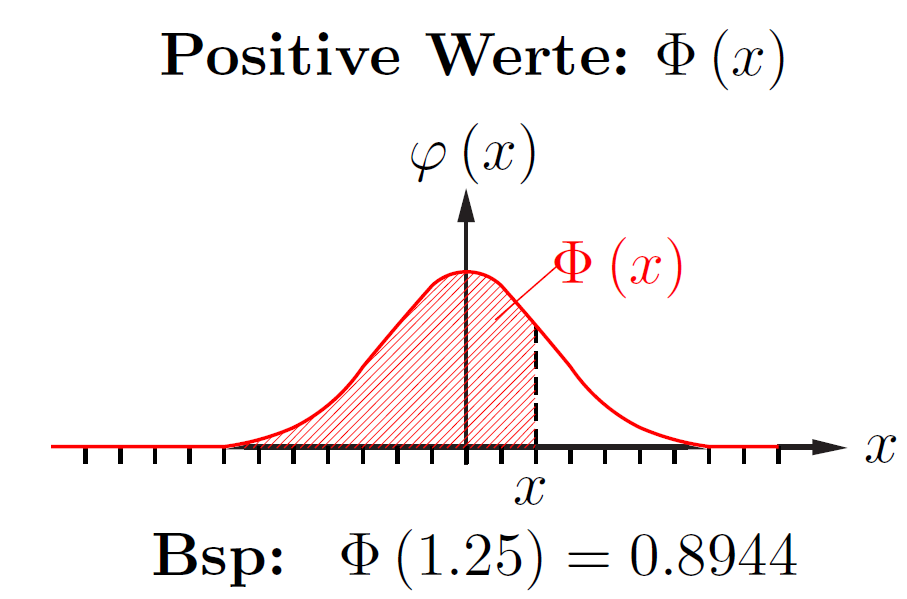
\includegraphics[width=45mm]{standardnormalverteilung_tabelle1.png}
\end{center}
\begin{center}
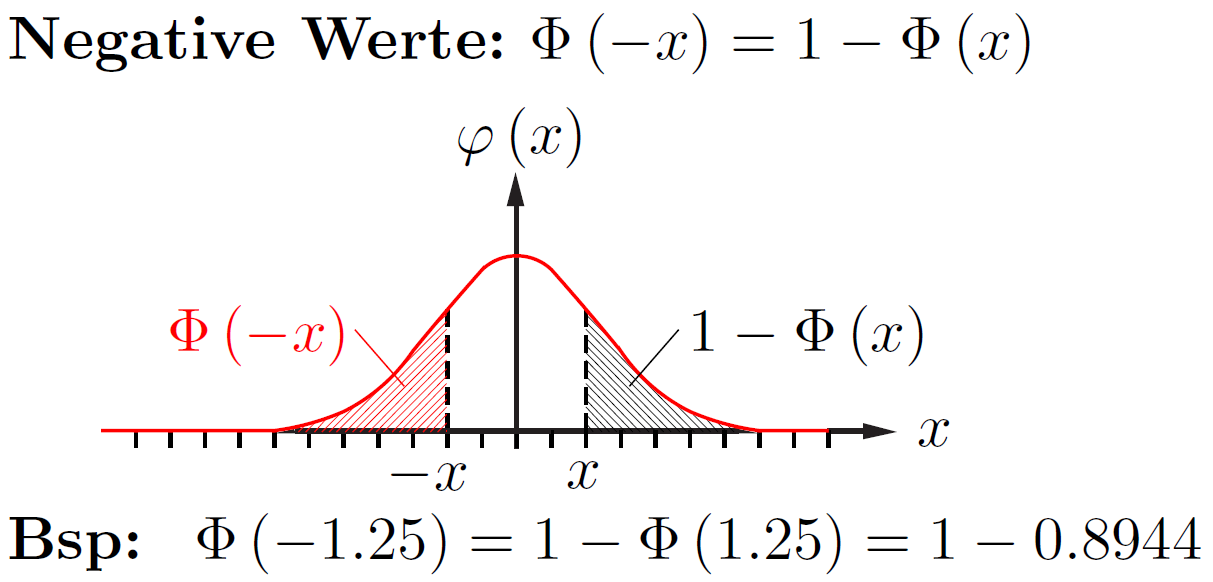
\includegraphics[width=60mm]{standardnormalverteilung_tabelle2.png}
\end{center}

Für nicht tabellierte Werte:
\[
\Phi^{-1}(0.03)=-\Phi^{-1}(0.97)=-1.88
\]

Regeln zum Auslesen der Werte:
\begin{itemize}
\item Ist ein gesuchter Wert $c$ nicht tabelliert, so wird derjenige Wert $a$ oder $b$ genommen, der näher bei $c$ liegt.
\item Sind zwei Werte $a$ und $b$ gleich weit vom gesuchten Wert $c$ entfernt, so wird der Mittelwert von $a$ und $b$ verwendet.
\end{itemize}

\subsection{Pareto-Verteilung}
Die Pareto-Verteilung, ist eine stetige Wahrscheinlichkeitsverteilung auf einem rechtsseitigen unendlichen Intervall $[x_0, \infty)$. Eine stetige Zufallsvariable $X$ heisst pareto-verteilt $Par(\alpha, x_0)$ mit den Parametern $\alpha > 0$ und $x_0 > 0$, mit folgenden Eigenschaften:

\vspace{10pt}

Notation:
\[
X \sim Par(\alpha, x_0)
\]

Dichtefunktion:
\[
f(x) =\begin{cases}
			\dfrac{\alpha}{x_0}\left(\dfrac{x_0}{x}\right)^{\alpha + 1} & x \geq x_0\\
			0 & x < x_0
		\end{cases}
\]

Verteilungsfunktion:
\[
F(x; x_0, \alpha) = \begin{cases}
			1 - \left(\dfrac{x}{x_0}\right)^{-\alpha} & x \geq x_0, \alpha > 0,\\
			0 & \text{sonst}
		\end{cases}
\]

Erwartungswert:
\[
E[X] = \begin{cases}
			x_0\dfrac{\alpha}{\alpha - 1} & \alpha > 1\\
			\infty & \alpha \leq 1
		\end{cases}
\]

Varianz:
\[
Var[X] = \begin{cases}
			x_0^2 \left(\dfrac{\alpha}{\alpha - 2} - \dfrac{\alpha^2}{(\alpha - 1)^2}\right)\\
			= x_0^2 \dfrac{\alpha}{(\alpha - 2)(\alpha - 1)^2} & \alpha > 2\\
			\infty & \alpha \leq 2
		\end{cases}
\]

Standardabweichung:
\[
sd[X]=\dfrac{x_0}{\alpha - 1}\sqrt{\dfrac{\alpha}{\alpha - 2}} \text{ für } \alpha > 2
\]

\textbf{Beispiel:} Die Verteilung wurde zunächst zur Beschreibung der Einkommensverteilung Italiens verwendet. Paretoverteilungen finden sich charakteristischerweise dann, wenn sich zufällige, positive Werte über mehrere Größenordnungen erstrecken und durch das Einwirken vieler unabhängiger Faktoren zustande kommen.

\section{Grenzwertsätze}
In vielen Situationen taucht die Summe von \emph{vielen gleichartigen Zufallsvariablen} auf. Wir möchten wissen, wie sich diese Summe etwa verhält, und untersuchen deshalb ihre Asymptotik, wenn die Anzahl der Summanden gegen unendlich geht.

Für die folgenden Sätze definieren wir einige Grössen:\\
$S_n=\sum\limits_{i=1}^{n}X_i$ und $\overline{X}_n=\frac{S_n}{n}=\frac{1}{n}\sum\limits_{i=1}^{n}X_i$

\subsection{Schwaches Gesetz der grossen Zahlen}
Seien $X_1,X_2,...,X_n$ \emph{unabhängige} oder \emph{paarweise unkorrelierte} Zufallsvariablen mit gleichem Erwartungswert $E[X_i]=\mu$ und gleicher Varianz $Var[X_i]=\sigma^2$. Sei $\overline{X}_n=\frac{1}{n}\sum\nolimits_{i=1}^{n}X_i$. Dann gilt:
\[
\forall\epsilon>0:\lim_{n\to\infty}P\left[|\overline{X}_n-\mu|>\epsilon\right]=0
\]

\textbf{Bemerkungen:}
\begin{itemize}
\item Für hinreichend grosse $n$ konvergiert der Mittelwert $\overline{X}_n$ gegen den Erwartungswert $\mu$.
\item Der Satz funktioniert nicht, falls der Erwartungswert oder die Varianz nicht definiert sind.
\end{itemize}

\subsection{Starkes Gesetz der grossen Zahlen}
Seien $X_1,...,X_n$ \emph{unabhängige} Zufallsvariablen mit \emph{gleicher Verteilung} (i.i.d) und Erwartungswert $E[X_i]=\mu$. Sei $\overline{X}_n=\frac{1}{n}\sum\nolimits_{i=1}^{n}X_i$. Dann gilt:
\[
P\left[\lim_{n\to\infty}\overline{X}_n=\mu\right]=1
\]

\textbf{Bemerkungen:}
\begin{itemize}
\item Für hinreichend grosse $n$ konvergiert der Mittelwert $\overline{X}_n$ gegen den Erwartungswert $\mu$.
\end{itemize}

\subsection{Zentraler Grenzwertsatz}
$X_1,X_2,X_3,...,X_n,...$ seien \emph{stochastisch unabhängige} Zufallsvariablen, die alle der \emph{gleichen} Verteilungsfunktion mit Erwartungswert $\mu$ und Varianz $\sigma^2$ genügen. Dann konvergiert die Verteilungsfunktion $F_Z(u)$ der standardisierten Zufallsvariablen
\[
Z_n=\frac{(X_1+X_2+...+X_n)-n\mu}{\sqrt{n}\sigma}
\]
im Grenzfall $n\rightarrow\infty$ gegen die Verteilungsfunktion $\Phi(t)$ der Standardnormalverteilung:
\[
\lim_{n\to\infty}F_Z(u)=\Phi(u)=\frac{1}{\sqrt{2\pi}}\cdot\int\limits_{0}^{u}e^{-\frac{t^2}{2}}dt
\]

\textbf{Bemerkungen:}
\begin{itemize}
\item Für ein hinreichend grosses $n$ ist $Z_n=X_1+X_2+...+X_n$ annähernd \emph{normalverteilt} mit Erwartungswert $E[Z_n]=n\mu$ und Varianz $Var[Z_n]=n\sigma^2$.
\end{itemize}

\section{Statistik}

\subsection{Schätzer}
Schätzer sind Funktionen von Zufallsvariablen und somit selbst wieder Zufallsvariablen. Sie verfügen deshalb über einen Erwartungswert und eine Varianz.

\subsubsection{Erwartungstreuer Schätzer}
Ein Schätzer $T$ ist \emph{erwartungstreu} wenn der Erwartungswert des Schätzers gleich dem zu schätzenden Parameter $\vartheta$ ist:
\[
E_\vartheta [T] = \vartheta
\]

\subsubsection{Konsistenter Schätzer}
Ein Folge von Schätzern $T^{(n)}$ ist \emph{konsistent} wenn diese mit zunehmendem Stichprobenumfang $n$ gegen den gesuchten Parameter $\vartheta$ konvergiert:
\[
\lim_{n\to\infty}P_{\vartheta}\left[|T^{(n)}-\vartheta| > \epsilon\right] = 0\text{ (für jedes $\epsilon > 0$)}
\]

\subsubsection{Momenten-Methode}
Sei $X_1,X_2,...,X_n$ eine Stichprobe vom Umfang $n$ mit gegebener Verteilung $t$. Die Parameter von $t$ seien unbekannt. Mit der Momenten-Methode können diese geschätzt werden. Der Momentenschätzer ist i.d.R. nicht erwartungstreu.

\vspace{10pt}

\textbf{Vorgehen:}
\begin{enumerate}
\item 1. Moment berechnen:
\[
\overline{x} = \frac{1}{n}\sum\limits_{i=1}^{n}x_i
\]
\item 2. Moment berechnen:
\[
s^2 = \frac{1}{n}\sum\limits_{i=1}^{n}\left(x_i - \overline{x}\right)^2=\left( \frac{1}{n}\sum\limits_{i=1}^{n}x_i^2\right)-\overline{x}^2
\]
\item Nimm die Formel für den Erwartungswert der geg. Verteilung $t$ und setze sie gleich $\overline{x}$
\item Nimm die Formel für die Varianz der geg. Verteilung $t$ und setze sie gleich $s^2$
\item Löse das Gleichungssystem auf. Du erhälst die gesuchten Parameter.
\end{enumerate}

\subsubsection{Maximum-Likelihood-Methode}
Methode zur systematischen Gewinnung von Schätzfunktionen.

\vspace{10pt}

\textbf{Vorgehen:}
\begin{enumerate}
\item Likelihood-Funktion aufstellen:
\[
L(x_1,...,x_n,\vartheta)= \prod \limits_{i=1}^{n} f(x_i,\vartheta)
\]
\item Log-Likelihood-Funktion aufstellen (logarithmieren von $L$):
\[
\log L(x_1,...,x_n,\vartheta)
\]
\item $\log L$ mit Hilfe elementarer Logarithmenregeln möglichst vereinfachen
\item $\log L$ nach jedem unbekannten Parameter partiell ableiten
\item Partielle Ableitungen = 0 setzen
\item Gleichungssystem nach Parametern auflösen
\end{enumerate}

\subsection{Tests}

\subsubsection{Wichtige Begriffe}

\begin{itemize}
\item \textbf{Nullhypothese $H_0$:} Die zu prüfende Annahme.
\item \textbf{Alternativhypothese $H_A$}: Alternative Annahme, falls $H_0$ verworfen werden muss.
\item \textbf{Signifikanzniveau $\alpha$}: Ist die Wahrscheinlichkeit, dass die Nullhypothese verworfen werden muss (auch Wahrscheinlichkeit für Fehler 1. Art).
\item \textbf{Teststatistik T:} Test- oder Prüfwert.
\item \textbf{P-Wert:} Das kleinste Niveau, auf dem der Test die Nullhypothese noch verwirft.
\item \textbf{Fehler 1. Art:} $H_0$ wird verworfen, obwohl sie richtig wäre.
\item \textbf{Fehler 2. Art:} $H_0$ wird beibehalten, obwohl $H_A$ stimmt.
\end{itemize}

\subsubsection{Allgemeines Vorgehen}
\begin{enumerate}
\item Wahl des Modells
\item Formulieren von $H_0$ und $H_A$.
\item Signifikanzniveau $\alpha$ festlegen.
\item Teststatistik T $T$ festlegen.
\item Bestimmen der kritischen Grenzen.
\item Konkreter Wert für Teststatistik $T$ berechnen.
\item Testentscheidung: $H_0$ beibehalten oder verwerfen?
\end{enumerate}

\subsubsection{z-Test}
Der z-Test ist ein Test für den Erwartungswert bei \emph{bekannter} Varianz $\sigma^2$. Es seien also $X_1,X_2,...,X_n \sim N(\vartheta,\sigma^2)\ i.i.d.$. Wir wollen die Nullhypothese $\vartheta=\vartheta_0$ testen.

\[
\begin{array}{ll}
	\text{Mittelwert $\overline{X}$:} & \overline{X}=\frac{X_1+X_2+...+X_n}{n} \\
	\text{Teststatistik $T$:} & T = \frac{\overline{X}-\vartheta_0}{\sigma/\sqrt{n}}\sim N(0,1) \\
\end{array}
\]

\textbf{Kritischer Bereich:} \\
Den kritischen Bereich bestimmt man abhängig von der Alternativhypothese $H_A$:
\begin{itemize}
\item $\vartheta_A > \vartheta_0$ einseitig: $K = (c_>,\infty)$ mit
\[
c_> = (1 - \alpha)\text{-Quantil} = \Phi^{-1}(1 - \alpha)
\]
\item $\vartheta_A < \vartheta_0$ einseitig: $K = (-\infty,c_<)$ mit
\[
c_< = \alpha\text{-Quantil} = \Phi^{-1}(\alpha)
\]
\item $\vartheta_A \neq \vartheta_0$ zweiseitig: $K = (-\infty,c_{\neq}) \cup (c_{\neq},\infty)$ mit
\[
c_{\neq} = \left(1-\frac{\alpha}{2}\right)\text{-Quantil} = \Phi^{-1}\left(1-\frac{\alpha}{2}\right)
\]
\end{itemize}

\subsubsection{t-Test}
Der t-Test ist ein Test für den Erwartungswert bei \emph{unbekannter Varianz} $\sigma^2$. Es seien also $X_1,X_2,...,X_n \sim N(\vartheta,\sigma^2) i.i.d.$. Wir wollen die Nullhypothese $\vartheta=\vartheta_0$ testen.

\[
\begin{array}{ll}
	\text{Mittelwert $\overline{X}$:} & \overline{X}=\frac{X_1+X_2+...+X_n}{n} \\
	\text{Schätzfunktion für $S^2$:} & S^2 = \frac{1}{n-1}\cdot \sum\limits_{i=0}^{n}(X_i - \overline{X})^2 \\
	\text{Teststatistik $T$:} & T = \frac{\overline{X}-\vartheta_0}{S/\sqrt{n}}\sim t_{n-1} \\
\end{array}
\]

Die Teststatistik $T$ ist \textbf{t-verteilt} mit \textbf{$n-1$ Freiheitsgraden}. Der kritische Bereich lässt sich analog zum z-Test mit den Quantilen der $t_{n-1}$-Verteilung bestimmen.

\subsubsection{Likelihood-Quotienten-Test}
Der Likelihood-Quotienten-Test kann man verwenden, um eine geeignete Teststatistik $T$ zu erhalten. 

\vspace{10pt}

\textbf{Vorgehen:}
\begin{enumerate}
\item Verallgemeinerter Likelihood-Quotient aufstellen:
\[
R(x_1,x_2,...,x_n;\vartheta_0,\vartheta_A):=\frac{L(x_1,x_2,...,x_n;\vartheta_0)}{L(x_1,x_2,...,x_n;\vartheta_A)}
\]
\item Formel vereinfachen. Im Exponent muss eine Summenformel stehen.
\item Überlegen, welcher Wert grösser ist, $\vartheta_0$ oder $\vartheta_A$?                  
\end{enumerate}

Ist dieser Quotient klein, sind die Beobachtungen für die Alternativhypothese deutlich wahrscheinlicher als für die Nullhypothese. Der Verwerfungsbereich $K:=[0,c)$ wird so gewählt, dass der Test das gewünschte Signifikanzniveau einhält.

\subsubsection{Ungepaarter Zweistichproben-z-Test}
Seien $X_1,X_2,...,X_n \sim N(\mu_X,\sigma^2)$ und $Y_1,Y_2,...,Y_n \sim N(\mu_Y,\sigma^2)$ zwei Stichproben mit $m = n$ oder $m \neq n$. Die Erwartungswerte $\mu_X$ und $\mu_Y$ seien unbekannt, die Varianz $\sigma^2$ sei \emph{bekannt}. Der Test kann wie ein normaler z-Test durchgeführt werden, als Teststatistik $T$ wird jedoch folgende Formel verwendet:
\[
T = \frac{\left(\overline{X}_n-\overline{Y}_m\right)-\left(\mu_X-\mu_Y\right)}{\sigma\sqrt{\frac{1}{n}+\frac{1}{m}}}\sim N(0,1)
\]

\subsubsection{Ungepaarter Zweichstichproben-t-Test}
Seien $X_1,X_2,...,X_n \sim N(\mu_X,\sigma^2)$ und $Y_1,Y_2,...,Y_n \sim N(\mu_Y,\sigma^2)$ zwei Stichproben mit $m = n$ oder $m \neq n$. Die Erwartungswerte $\mu_X$ und $\mu_Y$ seien unbekannt, die Varianz $\sigma^2$ sei ebenfalls \emph{unbekannt}. Der Test kann wie ein normaler t-Test durchgeführt werden, als Teststatistik $T$ wird jedoch folgende Formel verwendet:
\[
S_{X}^{2}=\frac{1}{n-1}\sum\limits_{i=1}^{n}\left(X_i-\overline{X}_n\right)^2
\]
\[
S_{Y}^{2}=\frac{1}{m-1}\sum\limits_{j=1}^{m}\left(Y_j-\overline{Y}_m\right)^2
\]
\[
S^2=\frac{1}{m+n-2}\left((n-1)S_{X}^{2}+(m-1)S_{Y}^{2}\right)
\]
\[
T = \frac{\left(\overline{X}_n-\overline{Y}_m\right)-\left(\mu_X-\mu_Y\right)}{S\sqrt{\frac{1}{n}+\frac{1}{m}}}\sim t_{n+m-2}
\]

\subsection{Konfidenzbereiche}
Ein Konfidenzbereich gibt ein Intervall an, in dem sich ein gesuchter Parameter mit sehr hoher Wahrscheinlichkeit befindet.




\section{Differentialrechnung}

\subsection{Faktorregel}
Ein konstanter Faktor bleibt beim Differenzieren erhalten:
\[
y=C\cdot f(x)\Rightarrow y'=C\cdot f'(x)
\]

\subsection{Summenregel}
Bei einer endlichen Summe von Funktionen darf gliedweise differenziert werden:
\[
y=f_1(x)+f_2(x)+...+f_n(x)\Rightarrow y'=f_1'(x)+f_2'(x)+...+f_n'(x)
\]

\subsection{Produktregel}
Die Ableitung einer in Produktform $y=u(x)\cdot v(x)$ darstellbaren Funktion erhält man nach folgender Produktregel:
\[
y'=u'(x)\cdot v(x)+u(x)\cdot v'(x)=u'v+uv'
\]

\subsection{Quotientenregel}
Die Ableitung einer Funktion, die als Quotient zweier Funktionen $u(x)$ und $v(x)$in der Form $y=\frac{u(x)}{v(x)}$ darstellbar ist, erhält man nach der Quotientenregel:
\[
y'=\frac{u'(x)\cdot v(x)-u(x)\cdot v'(x)}{v^2(x)}
\]

\subsection{Kettenregel}
Die Ableitung einer zusammengesetzten (verketteten) Funktion $y=F(u(x))=f(x)$ erhält man als Produkt aus äusserer und innerer Ableitung:
\[
y'=\frac{dy}{dx}=\frac{dy}{du}\cdot \frac{du}{dx}
\]

\subsection{Partielle Differentiation}
Summanden, die keine Variable beinhalten nach der abgeleitet wird, fallen WEG!

\subsection{Wichtige elementare Ableitungen}
\[
\begin{array}{lll}
	f(x)=c & \rightarrow & f'(x)=0 \\
	f(x)=x^n & \rightarrow & f'(x)=n\cdot x^{n-1} \\	
	f(x)=\sqrt{x}& \rightarrow & f'(x)=\frac{1}{2\sqrt{x}} \\
	f(x)=e^x & \rightarrow & f'(x)=e^x \\
	f(x)=a^x & \rightarrow & f'(x)=(\ln a)\cdot a^x \\
	f(x)=\ln x & \rightarrow & f'(x)=\frac{1}{x} \\
	f(x)=\log_{a}x & \rightarrow & f'(x)=\frac{1}{(\ln a)\cdot x} \\
\end{array}
\]

\section{Integralrechnung}

\subsection{Faktorregel}
Ein konstanter Faktor darf vor das Integral gezogen werden:
\[
\int\limits_{a}^{b}C\cdot f(x)dx=C\cdot\int\limits_{a}^{b}f(x)dx
\]

\subsection{Summenregel}
Eine endliche Summe von Funktionen darf giedweise integriert werden:
\[
\int\limits_{a}^{b}\left(f_1(x)+f_2(x)+...+f_n(x)\right)dx=
\]
\[
\int\limits_{a}^{b}f_1(x)dx+\int\limits_{a}^{b}f_1(x)dx+...+\int\limits_{a}^{b}f_1(x)dx
\]

\subsection{Vertauschungsregel}
Vertauschen der beiden Integrationsgrenzen bewirk einen Vorzeichenwechsel des Integrals:
\[
\int\limits_{a}^{b}f(x)dx=-\int\limits_{b}^{a}f(x)dx
\]

\subsection{Gleiche Integrationsgrenzen}
Fallen die Integrationsgrenzen zusammen ($a=b$), so ist der Integralwert gleich Null:
\[
\int\limits_{a}^{b}f(x)dx=0
\]

\subsection{Partielle Integration}
\[
\int f(x)dx=\int u(x)\cdot v'(x)dx=u(x)\cdot v(x)-\int u'(x)\cdot v(x)dx
\]

Vorgehen:
\begin{enumerate}
\item Integrand in $u(x)$ und $v'(x)$ zerlegen.
\item $u(x)$ ableiten, $v'(x)$ integrieren.
\item Formel aufschreiben und lösen.
\end{enumerate}

\subsection{Wichtige Stammintegrale}
\renewcommand*{\arraystretch}{2}
\[
\begin{array}{cc}

	\int x^ndx=\frac{x^{n+1}}{n+1}+C & \int a^xdx=\frac{a^x}{\ln a}+C \\
	\int\frac{1}{x}dx=\ln |x|+C & \int e^xdx=e^x+C \\
\end{array}
\]
\renewcommand*{\arraystretch}{1}

\subsection{Weitere Integrale}
\[
\begin{array}{rcll}
\int a\ dx & = & ax & \\
\int x^a\ dx & = & \frac{1}{a+1} x^{a+1} , & a \neq -1 \\
\int (ax+b)^c\ dx & = & \frac{1}{a(c+1)}(ax+b)^{c+1}, & c \neq -1 \\
\int \frac{1}{x}\ dx & = & \log\left|x\right|, & x\neq 0 \\
\int \frac{1}{ax+b}\ dx & = & \frac{1}{a} \log\left|ax+b\right| & \\
\int \frac{1}{x^2+a^2}\ dx & = & \frac{1}{a}\arctan\frac{x}{a} & \\
%
% EXPONENTIAL
%
\int e^{ax}\ dx & = & \frac{1}{a}e^{ax} & \\
\int x e^{ax}\ dx & = & \frac{e^{ax}}{a^2}(ax-1) & \\
\int x^2 e^{ax}\ dx & = & e^{ax}\left(\frac{x^2}{a}-\frac{2x}{a^2}+\frac{2}{a^3}\right) & \\
%
% LOGARITHMUS
%
\int \log\left|x\right|\ dx & = & x(\log\left|x\right| - 1) & \\
\int \log_a\left|x\right|\ dx & = & x(\log_a\left|x\right|-\log_a e) & \\
\int x^a \log x\ dx & = & \frac{x^{a+1}}{a+1}\left(\log x - \frac{1}{a+1}\right), & a\neq-1,x>0 \\
\int \frac{1}{x}\log x\ dx & = & \frac{1}{2}\log^2 x, & x>0 \\
\end{array}
\]

\section{Verschiedenes}
\textbf{Binomialkoeffizient} \\
Der Binomialkoeffizient
\[
\left(
\begin{array}{c}
	n \\
	k
\end{array}
\right)
\]
gibt für $n,k\in\mathbb{N}$ an, \textbf{wie viele Möglichkeiten es gibt, $k$ Objekte aus $n$ Objekten auszuwählen}. Damit gibt der Binomialkoeffizient an, wie viele $k$-elementige Teilmengen aus einer $n$-elementigen Menge gebildet werden können (gesprochen: ''k aus n'' oder ''k tief n'').

\vspace{10pt}

Für $k=0$ ist der Binomialkoeffizient $1$:
\[
\left(
\begin{array}{c}
	n \\
	0
\end{array}
\right)=1
\]

Für $k=1$ ist der Binomialkoeffizient $n$:
\[
\left(
\begin{array}{c}
	n \\
	1
\end{array}
\right)=n
\]

Für $k>n$ ist der Binomialkoeffizient stets $0$.

\vspace{10pt}

\textbf{Gammafunktion}
\[
\Gamma(x) = \int\limits_{0}^{\infty}t^{x-1}e^{-t}dt=(x-1)!
\]

\vspace{10pt}

\textbf{Diverse Summenformeln}
\[
\sum\limits_{k=0}^{\infty}\frac{1}{k!}=e
\]
\[
\sum\limits_{k=0}^{\infty}\frac{\lambda^k}{k!}=e^{\lambda}
\]
\[
\sum\limits_{k=1}^{\infty}\frac{\lambda^k}{k!}=e^{\lambda}-1
\]
\[
\sum\limits_{i=0}^{n}i=\sum\limits_{i=1}^{n}i=\frac{n(n-1)}{2}
\]
\[
\sum\limits_{i=1}^{n}i^2=\frac{n\cdot (n+1)\cdot (2n+1)}{6}
\]
\[
\sum\limits_{i=0}^{\infty}a\cdot p^i=\sum\limits_{i=1}^{\infty}a\cdot p^{i-1}=\frac{a}{1-p}
\]

\vspace{10pt}

\textbf{Mitternachtsformel} \\
Formel zum Auflösen von allgemeinen quadratischen Gleichungen der Form $ax^2+bx+c=0$:
\[
x_{1,2} = \frac{-b\pm\sqrt{b^2-4ac}}{2a} 
\]

\textbf{Produkteformeln}
\[
\prod\limits_{k=m}^{n}a\cdot x_i = a^{n-m+1}\cdot\prod\limits_{k=m}^{n}x_i
\]

\vspace{10pt}

\textbf{Logarithmenregeln}
\[
\begin{array}{rcl}
	\log{(uv)} & = & \log{(u)}+\log{(v)} \\
	\log{(\frac{u}{v})} & = & \log{(u)}-\log{(v)} \\
	\log_b{(r)} & = & \frac{\log_a(r)}{\log_a{(b)}} \\
	\log_a{(u^k)} & = & k\cdot\log_a{(u)} \\
	\log_a{(\sqrt[n]{u})} & = & \log_a{(u^{\frac{1}{n}})}=\frac{1}{n}\cdot\log_a{(u)} \\
	\log_a{(a^b)} & = & b \\ 
	\log{1} & = & 0 \\
	\log_a{(a)} & = & 1 \\	
	\ln{e} & = & 1 \\
		
\end{array}
\]


\section{Beispiele}

\subsection{t-Test}
Ein Waschmittelhersteller bringt 5kg-Packungen in den Umlauf. Die Konsumentenschutzorganisation kauft 25 Packungen. Es ergibt sich ein Mittel von $\overline{X}=4.9kg$ und eine empirische Stichprobenvarianz $S^2 = 0.1kg^2$. Die einzelnen Gewichte seine durch unabhängige $N(\mu,\sigma^2)$ Zufallsvariablen beschrieben.

\begin{enumerate}
\item Wie lauten die Hypothesen $H_0$ und $H_A$?
\item Wie ist $(\overline{X}-5) / (S / 5))$ verteilt unter $H_0$?
\item Führen Sie den t-Test auf dem 5%-Niveau durch. Wie gross ist der P-Wert? Wird die Nullhypothese verworfen?
\item Berechnen Sie das 95\%-Vertrauensintervall für den in 3. beschriebenen Test.
\end{enumerate}

\vspace{10pt}

\textbf{Lösung:}
\begin{enumerate}
\item $H_0: \mu = 5, H_1: \mu < 5$
\item Verteilung: $\sim t_{5^2-1} = t_{24}$
\item $T_1 = \frac{\overline{X}-\mu_0}{S/\sqrt{n}} = -1.581$. Wir ermitteln das t-Quantil für $n-1 = 24$ Freiheitsgrade und $t^{-1}(\alpha) = t^{-1}(0.05) = t^{-1}(0.95) = 1.711$. Somit erhalten wir eine kritische Grenze von $c = -1.711$. Weil $T_1 = -1.581 > c$ ist, wird die Nullhypothese nicht verworfen.
\item ???
\end{enumerate}

\subsection{Likelihood-Quotienten-Test}
Sei $x_1,x_2,...,x_n$ eine Stichprobe vom Umfang $6$ und poissonverteilt mit dem unbekannten Parameter $\lambda$. Die Hypothesen seien:
\[
\begin{array}{rl}
H_0: & \lambda=\lambda_0=0.5 \\
H_A: & \lambda=\lambda_A>\lambda_0 \\
\end{array}
\]
Die Teststatistik $T$ wird mit dem Likelihood-Quotienten ermittelt:
\[
R(x_1,...,x_6;\lambda_0,\lambda_A) =
\frac{
	L(x_1,x_2,...,x_6;\lambda_0)
}{
	L(x_1,x_2,...,x_6;\lambda_A)
} =
\]
\[
\frac{
	e^{-6\lambda_0}\prod\limits_{i=1}^{6}\frac{\lambda_{0}^{x_i}}{x_i!}
}{
	e^{-6\lambda_A}\prod\limits_{i=1}^{6}\frac{\lambda_{A}^{x_i}}{x_i!}
} =
e^{-6(\lambda_0-\lambda_A)}\left(\frac{\lambda_0}{\lambda_A}\right)^{\sum\limits_{i=1}^{6}x_i}
\]

Da $\lambda_0<\lambda_A$ wird $R(x_1,...,x_6;\lambda_0,\lambda_A)$ klein, genau dann, wenn $\sum\limits_{i=1}^{6}x_i$ gross ist. Statt des komplizierten Quotienten wählen wir als Teststatistik also
\[
T=\sum\limits_{i=1}^{6}X_i
\]

\subsection{Erwartungstreuer Schätzer}
Wir prüfen, ob der Schätzer $T = \frac{1}{n}\sum\limits_{i=1}^{n}X_i$ erwartungstreu ist.

\[
E[T] = E\left[\frac{1}{n}\sum\limits_{i=1}^{n}X_i\right] = \frac{1}{n}\sum\limits_{i=0}^{n}E[X_i] = \frac{1}{n} \cdot n \cdot \mu = \mu
\]

Der Schätzer $T$ ist erwartungstreu.

\subsection{Verteilung der Summe zweier normalerverteilter ZV}
Seien $X\sim N(\mu_1,\sigma_1^2)$ und $Y\sim N(\mu_2,\sigma_2^2)$. Wie ist $Z=1+aX+bY$ verteilt?

\vspace{10pt}

\textbf{Lösung:} \\
\[
\begin{array}{rcl}
	Z & \sim & N(1+aE[X]+bE[Y],a^2Var[X]+b^2Var[Y]) \\
	& \sim & N(1+a\mu_1+b\mu_2,a^2\sigma_1^2+b^2\sigma_2^2) \\
\end{array}
\]

\end{document}